%% LyX 2.3.3 created this file.  For more info, see http://www.lyx.org/.
%% Do not edit unless you really know what you are doing.
\documentclass[english]{article}
\usepackage[T1]{fontenc}
\usepackage{float}
\usepackage{amsmath}
\usepackage{graphicx}

\makeatletter

%%%%%%%%%%%%%%%%%%%%%%%%%%%%%% LyX specific LaTeX commands.
%% Because html converters don't know tabularnewline
\providecommand{\tabularnewline}{\\}

\makeatother

\usepackage{babel}
\begin{document}
\title{Homework 1}
\author{Zachary Taylor,John Dinofrio, Cristian Bueno}
\maketitle

\part*{Problem 1}

\textbf{Here, we aim to improve the quality of the video sequence provided above. This is a video recording of a highway during night. Most of the Computer Vision pipelines for lane detection or other self-driving tasks require good lighting conditions and color information for detecting good features. A lot of pre-processing is required in such scenarios where lighting conditions are poor. Now, using the techniques taught in class your aim is to enhance the contrast and improve the visual appearance of the video sequence. You can use any in-built functions for the same.}

The first approach we took to solve this problem was using the histogram equalization technique. Initially we made each frame grayscale and then equalized, but we also separated the three color channels, equalized each individually, and merged them back together into one image. 
\begin{figure}[H]
\begin{centering}
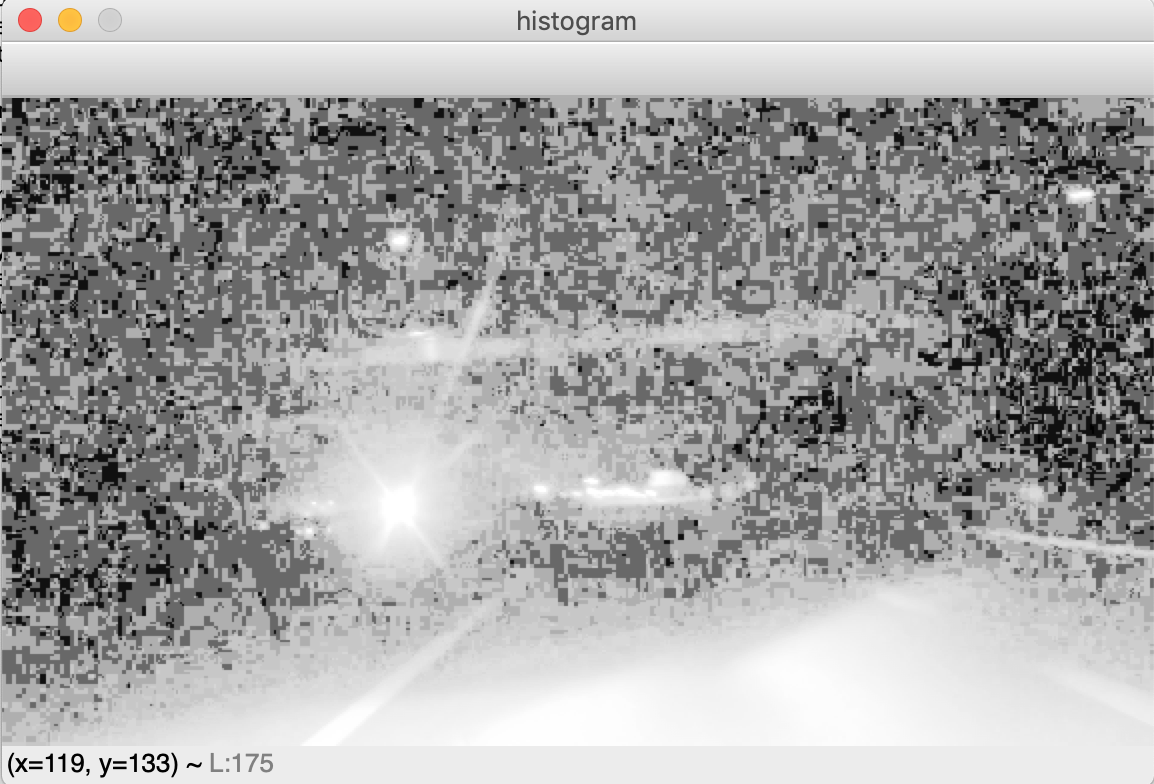
\includegraphics[viewport=0bp 0bp 500bp 461bp,angle=0,origin=c,scale=0.3]{./images/gray.png}
\par
\begin{tiny}
Histogram Equalized grayscale image
\end{tiny}
\end{centering}
\end{figure}

\end{document}
